\setchapterpreamble[u]{\margintoc}
\chapter{Վեկտորներ}
\labch{vectors}

\emergencystretch 2em

\section{Ներածություն}

Պատկերացրեք՝ ունեք $2$ հատ $10$ դրամանոց, $1$ հատ $20$ դրամանոց, $2$ հատ $50$ դրամանոց և $1$ հատ $200$ դրամանոց։ Ինչպե՞ս կարող ենք գրի առնել այդ փաստը։

Մի տարբերակ է՝ վերցնել ու աղյուսակով իրար տակ գրել յուրաքանչյուր մետաղադրամի արժեքը և մեր ունեցած քանակը․%\sidenote{Թեև $100$ դրամանոց չունենք, բայց ամեն դեպքում ավելացնենք նաև $100$-անոցի տողը․ միգուցե ինչ-որ պահի ունենանք։}
\begin{table}[h]
  % \centering
  \raggedright
  \begin{tabular}{|c|c|}
    \hline
    \textbf{արժեք} & \textbf{քանակ} \\
    \hline
    $10$ & $2$\\
    \hline
    $20$ & $1$\\
    \hline
    $50$ & $2$ \\
    \hline
    $100$ & $0$ \\
    \hline
    $200$ & $1$ \\
    \hline
  \end{tabular}
\end{table}

կամ, պարզապես, վերցնել այդ աղյուսակի երկու սյուները՝
\[
\begin{bmatrix}
10 \\ 20 \\ 50 \\ 100 \\ 200
\end{bmatrix}, \qquad \qquad \begin{bmatrix}
2 \\1 \\2 \\0 \\1 \\
\end{bmatrix}
\]

Վերևում գրված մի քանի թվերից բաղկացած օբյեկտներն անվանում ենք \textit{վեկտորներ։}

\begin{definition}
Իրական թվերի կարգավորված $n$-յակը\marginnote{կարգավորված $n$-յակ = ֆիքսված հեր\-թա\-կա\-նությամբ իրար կողք գրված $n$ հատ թիվ} կոչվում է \textbf{վեկտոր} (կամ \textbf{սյուն վեկտոր})՝
\[
\mathbf{v} = \begin{bmatrix} v_1 \\ v_2 \\ \vdots \\ v_n \end{bmatrix}
\]
իսկ \( v_1, v_2, \ldots, v_n \) թվերը կոչվում են վեկտորի \textbf{բաղադրիչներ}։
\end{definition}

Եթե նույն վեկտորը գրենք շրջած տեսքով՝ հորիզոնական, ապա կստանանք (ինչպես գուշակեցիք) \textit{տող վեկտոր՝}
\[\mathbf{v} = \begin{bmatrix} v_1 & v_2 & \ldots & v_n \end{bmatrix}։\]
$n$-չափանի բոլոր վեկտորների բազմությունը նշանակում ենք \( \mathbb{R}^n\)-ով։ Եթե նկատի ունենք, որ $\mathbf{v}$-ն \( \mathbb{R}^n \)-ից (այսինքն՝ $n$-չափանի) վեկտոր է, ապա գրում ենք՝ $\mathbf{v} \in \mathbb{R}^n$։

% \begin{exercise}
% Prove (or disprove) the Riemann hypothesis.
% \end{exercise}

Մասնավորապես, $\mathbb{R}^1$-ի վեկտորները հենց թվերն են՝ $[v]\in\mathbb{R}$:

\begin{example} 
Սրանք բոլորը համապատասխան չափանի վեկտորներ են՝
 \begin{align*}
    \mathbf{v}_1 &= \begin{bmatrix} 2 \\ -1 \\ 0 \end{bmatrix} \in \R^3 \\
    \mathbf{v}_2 &= \begin{bmatrix} 1 \\ 1 \\ 1 \\ 1 \end{bmatrix} \in \R^4 \\
    \mathbf{v}_3 &= \begin{bmatrix} -3 \\ 2 \end{bmatrix}\in \R^2 \\
    \mathbf{v}_4 &= \begin{bmatrix} 0 \\ 0 \\ 0 \end{bmatrix} \in \R^3 \\
    \mathbf{v}_5 &= \begin{bmatrix} 1 & -1 & 2 \end{bmatrix} \in \R^3
  \end{align*}
$\mathbf{v}_4$-ը կոչվում է $\R^3$ տարածության \textit{զրոյական վեկտոր} և նշանակվում թավ $0$-ով՝ $\mathbf{0}$։
\end{example}


 
\section{Գործողություններ վեկտորների հետ}

Նշանակենք 
\[
\mathbf{a} = \begin{bmatrix}
10 \\ 20 \\ 50 \\ 100 \\ 200
\end{bmatrix}, \qquad \mathbf{b} = \begin{bmatrix}
2 \\1 \\2 \\0 \\1 \\
\end{bmatrix}
\]
Այսպիսով՝
 $\mathbf{a}$, $\mathbf{b} \in \mathbb{R}^5$:
 
Պատկերացրեք՝ ինչ-որ մեկը մեզ տվեց, ասենք, $3 \times 100$ դրամ և ${1 \times 200}$ դրամ։ Նշանակենք
\[
\mathbf{c} = \begin{bmatrix}
0 \\ 0 \\ 0 \\ 3 \\ 1
\end{bmatrix}
\]
Այդ դեպքում կունենանք հետևյալ մետաղադրամները՝
\[
\mathbf{b} + \mathbf{c} = \begin{bmatrix}
2 \\1 \\2 \\0 \\1 \\
\end{bmatrix} + \begin{bmatrix}
0 \\ 0 \\ 0 \\ 3 \\ 1
\end{bmatrix} = \begin{bmatrix}
2+0 \\ 1+0 \\ 2+0 \\ 0+3 \\ 1+1
\end{bmatrix} = \begin{bmatrix}
2 \\ 1 \\ 2 \\ 3 \\ 2
\end{bmatrix}
\]

Ավելի ընդհանուր, 
\newpage 
\begin{definition}
Երկու $n$-չափանի  \( \mathbf{v} = \begin{bmatrix} v_1 \\ v_2 \\ \vdots \\ v_n \end{bmatrix} \) և \( \mathbf{u} = \begin{bmatrix} u_1 \\ u_2 \\ \vdots \\ u_n \end{bmatrix} \) 
\textbf{վեկտոր\-ների գումար} կանվանենք
  \begin{align*}
    \mathbf{v} + \mathbf{u} &= \begin{bmatrix} v_1 + u_1 \\ v_2 + u_2 \\ \vdots \\ v_n + u_n \end{bmatrix}
  \end{align*}
վեկտորը, այսինքն՝ գումարում ենք համապատասխան բաղա\-դրիչ\-ները։
\end{definition}

\warning{Տարբեր չափանի վեկտորներ իրար գումարել չենք կարող։}

Իսկ ի՞նչ, եթե ինչ-որ հրաշքով մետաղադրամները կրկնապատկվեին: Յուրաքանչյուր մետաղադրամից կունենայինք՝
$$2 \cdot \mathbf{b} = 2\cdot \begin{bmatrix}
2 \\1 \\2 \\0 \\1 \\
\end{bmatrix} = \begin{bmatrix}
4 \\2 \\4 \\0 \\2 \\
\end{bmatrix} $$
հատ։ Ուրեմն սահմանենք՝ 
\begin{definition}
Ցանկացած \( \mathbf{v} = \begin{bmatrix} v_1 \\ v_2 \\ \vdots \\ v_n \end{bmatrix} \) վեկտորի և  $c\in\R$ թվի\marginnote{թիվ բառի փոխարեն կօգտագործենք նաև \textit{սկալյար} {\it (scalar)} բառը} համար \textbf{$\mathbf{v}$ վեկտորի բազմապատկում $c$ թվով} կանվանենք
  \begin{align*}
    c \cdot \mathbf{v} &= \begin{bmatrix} c \cdot v_1 \\ c \cdot v_2 \\ \vdots \\ c \cdot v_n \end{bmatrix}
  \end{align*}
վեկտորը, այսինքն՝ $\mathbf{v}$-ի բոլոր բաղադրիչները բազմապատկում ենք $c$-ով։
\end{definition}

Ինչպես թվերի գումարում-բազմապատկումը, այնպես էլ վեկտորների գումարման և թվով բազմապատկման գործողությունները օժտված են հետևյալ լավ հատկություններով՝
\begin{itemize}
    \item զուգորդականություն, այսինքն՝
    \[
      (\mathbf{u} + \mathbf{v}) + \mathbf{w} = \mathbf{u} + (\mathbf{v} + \mathbf{w}) \quad  \text{ և } \quad
     (c \cdot d) \cdot \mathbf{v} = c \cdot (d \cdot \mathbf{v})
    \]

    \item տեղափոխականություն, այսինքն՝
        \[
     \mathbf{u} + \mathbf{v} = \mathbf{v} + \mathbf{u} \quad  \text{ և } \quad
     c \cdot (d \cdot \mathbf{v}) =  d \cdot (c \cdot \mathbf{v}) = (cd) \cdot \mathbf{v}
    \]

    \item բաշխականություն, այսինքն՝
    \[
     c \cdot (\mathbf{v} + \mathbf{u}) = c \cdot \mathbf{v} + c \cdot \mathbf{u}
    \]
\end{itemize}
ցանկացած  $\mathbf{u}$, $\mathbf{v} \in  \mathbb{R}^n$ վեկտորների և $c$, $d\in \R$ թվերի համար։

Վերջապես պատկերացրեք, որ մտնում եք խանութ և ծախսում ${2 \times 50}$ դրամանոց։ Ինչպե՞ս կփոխվի Ձեր գրպանի պարունակությունը։

\begin{definition}
Ցանկացած \( \mathbf{v} = \begin{bmatrix} v_1 \\ v_2 \\ \vdots \\ v_n \end{bmatrix} \) վեկտորի \textbf{հակադիր} կանվանենք
  \begin{align*}
     -\mathbf{v} &= \begin{bmatrix} -v_1 \\ -v_2 \\ \vdots \\ -v_n \end{bmatrix}
  \end{align*}
վեկտորը, այսինքն՝ $\mathbf{v}$ բոլոր բաղադրիչները բազմապատկում ենք $-1$-ով։
\end{definition}

Իսկ հակադիրի միջոցով սահմանենք վեկտորների հանումը՝
\begin{definition}
Երկու $n$-չափանի  \( \mathbf{u} = \begin{bmatrix} u_1 \\ u_2 \\ \vdots \\ u_n \end{bmatrix} \) և  \( \mathbf{v} = \begin{bmatrix} v_1 \\ v_2 \\ \vdots \\ v_n \end{bmatrix} \) 
\textbf{վեկտոր\-ների տարբերություն} կանվանենք $\vu$-ի և $-\mathbf{v}$-ի գումարը՝
  \begin{align*}
    \mathbf{v} + \mathbf{u} &= \begin{bmatrix} v_1 + u_1 \\ v_2 + u_2 \\ \vdots \\ v_n + u_n \end{bmatrix}
  \end{align*}
այսինքն՝ հանում ենք համապատասխան բաղադրիչները։
\end{definition}

\warning{Տարբեր չափանի վեկտորներ իրարից հանել չենք կարող։}

\begin{example}
    \[
    \begin{bmatrix} 2 \\ -1 \\ 3 \end{bmatrix} - \begin{bmatrix} 1 \\ 4 \\ 0 \end{bmatrix} = \begin{bmatrix} 2 - 1 \\ -1 - 4 \\ 3 - 0 \end{bmatrix} = \begin{bmatrix} 1 \\ -5 \\ 3 \end{bmatrix}
    \]
\end{example}


\section{Վեկտորների շրջումը}

Երբեմն ունենում ենք, ենթադրենք, $\mathbf{v}=\begin{bmatrix}
    3 \\ 4
\end{bmatrix}$ վեկտորը և ցանկանում ենք ինչ-որ ձևով նշանակել $\begin{bmatrix}
    3 & 4
\end{bmatrix}$ վեկտորը, այսինքն՝ որպես սյուն գրված վեկտորը գրել որպես տող։ Այդ դեպքում կգրենք պարզապես, որ
\[
\mathbf{v}^T = \begin{bmatrix}
    3 \\ 4
\end{bmatrix}^T = \begin{bmatrix}
    3 & 4
\end{bmatrix}
\]

\begin{definition}
\( \mathbf{v} = \begin{bmatrix} v_1 \\ v_2 \\ \vdots \\ v_n \end{bmatrix} \) սյուն \textbf{վեկտորի տրանսպոնացված} (կամ \textbf{շրջած}) ենք անվանում
\begin{align*}
\mathbf{v}^T = \begin{bmatrix} v_1 & v_2 & \cdots & v_n \end{bmatrix}
\end{align*}
տող վեկտորը, այսինքն՝ նույն $\mathbf{v}$-ն, բայց շրջած։
\end{definition}
Նույն ձևով սահմանում ենք տող վեկտորի տրանսպոնացվածը՝ որպես համապատասխան սյուն վեկտոր։ 

\begin{example}
 \[
    \begin{bmatrix} 2 \\ -1 \\ 3 \end{bmatrix}^T = \begin{bmatrix} 2 & -1 & 3 \end{bmatrix}
    \]
    \[
    \begin{bmatrix} 1 & 0 & -2 \end{bmatrix}^T = \begin{bmatrix} 1 \\ 0 \\ -2 \end{bmatrix}
    \]
\end{example}

Նկատենք, որ ցանկացած $c$ թվի և $\mathbf{v}$ վեկտորի համար 
\[
(c \cdot \mathbf{v})^T = c \cdot \mathbf{v}^T 
\]

\question{Ի՞նչ եք կարծում, ինչի՞ է հավասար $(\mathbf{v}^T)^T $-ն։}

Ինչպես տեսնում եք, տող և սյուն վեկտորների միջև էական տարբե\-րու\-թյուն չկա․ գրելաձևը տարբեր է, բայց բովանդակությունը՝ թվերը նույնն են։ Այնպես որ այսուհետև վեկտորների մասին խոսելիս չենք նշի «տող վեկտոր» կամ «սյուն վեկտոր», այլ պարզապես կասենք «վեկտոր»։

\warning{Տող վեկտորին սյուն վեկտոր գումարել չի կարելի:}


\section{Սկալյար արտադրյալ}

Վերադառնանք մեր մետաղադրամներին։ Ունեինք $\mathbf{a} = \begin{bmatrix}
10 \\ 20 \\ 50 \\ 100 \\ 200
\end{bmatrix}$  արժո\-ղու\-թյամբ  $\mathbf{b} = \begin{bmatrix}
2 \\1 \\2 \\0 \\1 \\
\end{bmatrix}$ քանակով մետաղադրամներ։

\question{Որքա՞ն գումար ունենք ընդհանուր։}

\begin{definition}
\( \mathbf{u} = \begin{bmatrix} u_1 \\ u_2 \\ \vdots \\ u_n \end{bmatrix} \) և \( \mathbf{v} = \begin{bmatrix} v_1 \\ v_2 \\ \vdots \\ v_n \end{bmatrix} \) վեկտորների \textbf{սկալյար արտադրյալ} կանվանենք
\[
\mathbf{u} \cdot \mathbf{v} = u_1 \cdot v_1 + u_2 \cdot v_2 + \cdots + u_n \cdot v_n
\]
թիվը։
\end{definition}
\begin{example}
Եթե  \( \mathbf{u} = \begin{bmatrix} 2 \\ -1 \\ 3 \end{bmatrix} \) և \( \mathbf{v} = \begin{bmatrix} 1 \\ 4 \\ 0 \end{bmatrix} \), ապա
    \[
    \mathbf{u} \cdot \mathbf{v} = (2 \cdot 1) + (-1 \cdot 4) + (3 \cdot 0) = 2 - 4 + 0 = -2
    \]
\end{example}

Մեր ունեցած գումարը պարզելու համար կարող ենք հաշվել արժո\-ղու\-թյուն\-ների ու քանակների  $\mathbf{a}$ և $ \mathbf{b}$ վեկտորների սկալյար արտադրյալը՝
$$\mathbf{a} \cdot \mathbf{b}= \begin{bmatrix}
2 \\1 \\2 \\0 \\1 \\
\end{bmatrix}\cdot \begin{bmatrix}
10 \\ 20 \\ 50 \\ 100 \\ 200
\end{bmatrix} = 2 \cdot 10 + 1 \cdot 20 + 2 \cdot 50 + 0 \cdot 100 + 1\cdot 200 = 340 $$

Նկատենք, որ եթե երկու վեկտորների գումարը կամ տարբերությունը վեկտոր է, ապա դրանց սկալյար արտադրյալը \textit{թիվ է} (ինչի համար էլ կոչվում է \textit{սկալյար} արտադրյալ)։ Իսկ քանի որ սկալյար արտադրյալը նշանակում են կետիկով՝ $\va \cdot \vb$, անգլերենում այն կոչվում է նաև {\it dot product:}

\warning{Սկալյար արտադրյալը սահմանված է միայն նույն չափանի վեկտորների համար։}

Ինչպես գումարման և թվով բազմապատկման դեպքում, սկալյար արտադրյալը ևս օժտված է օգտակար հատկություններով․
\begin{itemize}
  \item տեղափոխականություն՝ $$ \mathbf{u} \cdot \mathbf{v} = \mathbf{v} \cdot \mathbf{u}$$
  \item զուգորդականություն՝ $$(c \cdot \mathbf{u}) \cdot \mathbf{v} = c \cdot (\mathbf{u} \cdot \mathbf{v}) = \mathbf{u} \cdot (c \cdot \mathbf{v})$$
  \item բաշխականություն՝ $$ (\mathbf{u} + \mathbf{v}) \cdot \mathbf{w} = \mathbf{u} \cdot \mathbf{w} + \mathbf{v} \cdot \mathbf{w} $$
  \item դրական որոշյալություն՝ 
  $$\mathbf{u} \cdot \mathbf{u} \geq 0, $$
  ընդ որում զրոյի հավասարվելու միակ դեպքն այն է, երբ $\mathbf{u} = \mathbf{0}$:
\end{itemize}

\question{Ինչո՞ւ է չորրորդ հատկությունը ճիշտ ցանկացած վեկտորի համար։}


\begin{example}
Հաշվենք \( (5\mathbf{u} - \mathbf{v}) \cdot \mathbf{w} \) արտահայտության արժեքը
 \[ \mathbf{u} = \begin{bmatrix} 1 \\ -2 \\ 3 \end{bmatrix}, \qquad  \mathbf{v} = \begin{bmatrix} 0 \\ 4 \\ -1 \end{bmatrix}, \qquad \mathbf{w} = \begin{bmatrix} -2 \\ 1 \\ 2 \end{bmatrix} \]
 վեկտորների համար։

  \begin{align*}
      (5\mathbf{u} - \mathbf{v}) \cdot \mathbf{w} &= \left(5\cdot\begin{bmatrix} 1 \\ -2 \\ 3 \end{bmatrix} - \begin{bmatrix} 0 \\ 4 \\ -1 \end{bmatrix}\right) \cdot \begin{bmatrix} -2 \\ 1 \\ 2 \end{bmatrix} \\&= \left(\begin{bmatrix} 5 \\ -10 \\ 15 \end{bmatrix} - \begin{bmatrix} 0 \\ 4 \\ -1 \end{bmatrix}\right) \cdot \begin{bmatrix} -2 \\ 1 \\ 2 \end{bmatrix} 
      \\&= \begin{bmatrix} 5 \\ -14 \\ 16 \end{bmatrix} \cdot \begin{bmatrix} -2 \\ 1 \\ 2 \end{bmatrix} = 5 \cdot (-2) + (-14) \cdot 1 + 16 \cdot 2 = 8  \end{align*}
\end{example}

% \question{Իմաստ ունի՞ $u$։}


\section{Վեկտորների պատկերումը երկրաչափորեն}

Մինչ այս պահը վեկտորները մեր համար զուտ ինչ-որ թվացուցակներ են։ Պարզվում է, որ իրականում վեկտորներն ունեն շատ գեղեցիկ երկրաչափական մեկնաբանություն։ 

Վերցնենք օրինակ՝
\[
\vv=\begin{bmatrix}2\\3    \end{bmatrix}
\]
երկչափ վեկտորը։ Այն կարող ենք պատկերել հետևյալ ձևով․ վերցնենք կոորդինատական հարթության $(0, 0)$ սկզբնակետը և սլաքով միացնենք $(2, 3)$ կոորդինատներով կետին։

\begin{center}
  \begin{tikzpicture}[scale=1]
    \draw[->] (0,0) -- (2,3) node[midway, above left] {$\mathbf{v}$};
    \draw[dashed] (0,0) -- (2,0) node[midway, below] {$2$};
    \draw[dashed] (2,0) -- (2,3) node[midway, right] {$3$};
  \end{tikzpicture}
\end{center}

Արդյունքում կստանանք սլաք (կամ ուղղորդված հատված), որը հենց կլինի $\vv$ վեկտորի երկրաչափական պատկերը։ Այս եղանակով կարող ենք $\R^2$ տարածության բոլոր վեկտորների մասին մտածել որպես $(0, 0)$ կետից սկսվող որոշակի ուղղություն և երկարություն ունեցող \textit{սլաքների՝}
\[
\begin{bmatrix}
    x \\ y
\end{bmatrix} \quad \mapsto \quad (0,0)\text{-ից սկսվող սլաք դեպի }(x, y)
\]

Նման ձևով $\R^3$-ի վեկտորները նույնպես կարող ենք պատկերել որպես եռաչափ ({\rm 3D}) տարածության մեջ սլաքներ։ Ինչպես ընթացքում կտեսնենք, վեկտորներին առնչվող բազմաթիվ գաղափարներ բավարար է հասկանալ ընդամենը $2$-չափ ու $3$-չափ դեպքերում,\marginnote{2-3 բաժակ հետո հնարավոր է պատկե\-րել նաև $\R^4$-ի վեկտորները} որպեսզի պատկե\-րաց\-նենք, թե ինչ է տեղի ունենում ավելի մեծ չափանի տարածու\-թյուն\-նե\-րում։

Վեկտորները երկրաչափորեն պատկերելը օգտակար է հատկապես նրանով, որ այսպես ավելի հեշտ է պատկերացնել դրանց հետ կատարվող գործողությունները․

\begin{description}
\item[Գումարում․] Երկու $\mathbf{u}$ և $\mathbf{v}$ վեկտորներ գումարելու համար $\vv$ վեկտորի սկզբնակետը տեղադրում ենք $\vu$ վեկտորի վերջնակետից։ Արդյուն\-քում $\vu$-ի սկզբնակետից դեպի $\vv$-ի վերջնակետը ուղղված վեկտորը կլինի $\mathbf{u} + \mathbf{v}$-ն։

\begin{center}
  \begin{tikzpicture}[scale=0.8]
    \draw[->] (0,0) -- (2,3) node[midway, above left] {$\mathbf{u}$};
    \draw[->] (2,3) -- (5,1) node[midway, above right] {$\mathbf{v}$};
    \draw[->,myred] (0,0) -- (5,1) node[midway, below] {$\mathbf{u} + \mathbf{v}$};
  \end{tikzpicture}
\end{center}

\item[Հակադիր․] $\mathbf{v}$ վեկտորի $-\mathbf{v}$ հակադիրը այն վեկտորն է, որն ունի նույն երկարությունը և ուղղված է $\vv$-ին հակառակ։

    \begin{center}
      \begin{tikzpicture}[scale=0.8]
        \draw[->] (0,0) -- (3,2) node[midway, above left] {$\mathbf{v}$};
        \draw[->,myred] (0,0) -- (-3,-2) node[midway, below] {$\qquad -\mathbf{v}$};
      \end{tikzpicture}
    \end{center}

\item[Հանում․] $\mathbf{u}$ վեկտորից $\mathbf{v}$ վեկտորը հանելու համար կարող ենք $\vu$-ին գումարել $\vv$-ի հակադիրը, կամ ուրիշ կերպով՝ $\vu$-ն ու $\vv$-ն պատկերել միևնույն սկզբնակետից, ծայրակետերը միացնել իրար՝ ստանալով եռանկյուն, և վերցնել $\vv$-ի վերջնակետից դեպի $\vu$-ի վերջնակետն ուղղված վեկտորը։

\begin{center}
  \begin{tikzpicture}[scale=0.8]
    \draw[->] (0,0) -- (2,3) node[midway, right] {$\;\mathbf{u}$};
    \draw[->] (0, 0) -- (-3,2) node[midway, left] {$\mathbf{v}\quad $};
    \draw[->,myred] (-3,2) -- (2,3) node[midway, above] {$\mathbf{u} - \mathbf{v}$};
  \end{tikzpicture}
\end{center}


\item[Թվով բազմապատկում․] $\mathbf{v}$ վեկտորը $c$ դրական թվով բազմապատկելիս այն ձգվում/սեղմվում է $c$ անգամ, այսինքն՝ ստացվում է նույն ուղղությամբ, բայց տարբեր երկարությամբ վեկտոր։

\begin{center}
  \begin{tikzpicture}[scale=0.8]
    \draw[->] (0,0) -- (3,2) node[midway, above left] {$\mathbf{v}$};
    \draw[->,myred] (0,0) -- (6,4) node[near end, above left] {$2  \mathbf{v}$};
  \end{tikzpicture}
\end{center}

Բացասական $c$-ով բազմապատկելիս երկարությունը կրկին բազմապատկվում է $|c|$ անգամ, բայց վեկտորը շրջվում է հակառակ ուղղությամբ։
\end{description}


\question{Ի՞նչ է դառնում վեկտորը, երբ այն բազմապատկում ենք $0$-ով։}


\begin{example}
Եթե $\va = \begin{bmatrix} 3 & 2 \end{bmatrix}$ և $\vb = \begin{bmatrix} 2 & 0 \end{bmatrix}$, ապա $3\va+\vb$-ն գտնելու համար պետք է
\begin{enumerate}
    \item $\va$-ն ձգել $3$ անգամ,
    \item $\vb$-ն տեղադրել ստացված $3\va$ վեկտորի վերջնակետից,
    \item (լրացրու ինքդ)
\end{enumerate}

\begin{center}
\begin{tikzpicture}[scale=0.8]
  \draw[->] (0,0) -- (3,2) node[midway, above left] {$\mathbf{a}$};
  \draw[->] (0,0) -- (2,0) node[midway, below] {$\mathbf{b}$};
  \draw[->] (0,0) -- (9,6) node[midway, left] {$3\mathbf{a}\;\;\;$};
  \draw[->] (9,6) -- (11,6) node[midway, above] {$\mathbf{b}$};
  \draw[->,myred] (0,0) -- (11,6) node[midway, below] {\;\;\;\;\;\;\;\;$3\mathbf{a} + \mathbf{b}$};
\end{tikzpicture}
\end{center}
\end{example}

\section{Նորմ}

Վեկտորների երկրաչափական պատկերումից հարց է առաջանում․ եթե վեկտորը սլաք է, ապա ինչի՞ է հավասար նրա երկարությունը։ 
Դե, հատվածի երկարությունը նրա սկզբնակետի և վերջնակետի միջև եղած հեռավորությունն է։ Իսկ ինչպե՞ս հաշվենք այդ հեռավորությունը, օրինակ, $\begin{bmatrix}
    3 & 4
\end{bmatrix}$ վեկտորի դեպքում՝ օգտվելով դրա կոորդինատներից ($3$ և $4$ թվերից)։ 


\begin{figure}[h]
    \centering
    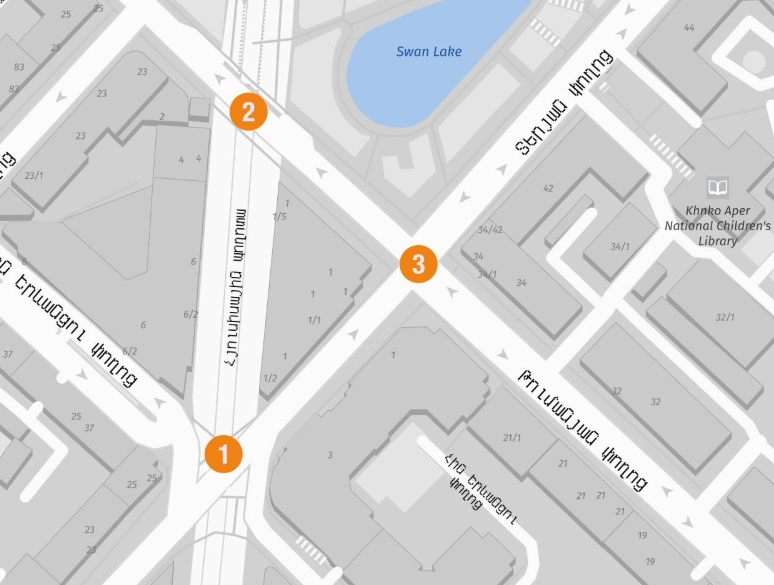
\includegraphics[width=0.75\linewidth]{chapters/chapter 1/evn_map.png}
\end{figure}

Որքա՞ն ճանապարհ պետք է անցնել, օրինակ, Հյուսիսային-Տերյան \circled{$1$} և Հյուսիսային-Թումանյան \circled{$2$} խաչմերուկների միջև։ 

\textbf{Հետիոտնի տեսանկյունից՝} \circled{$1$} և \circled{$2$} կետերի հեռավորությունը հավասար է դրանք միացնող հատվածի երկարությանը։

\textbf{Վարորդի տեսանկյունից՝} \circled{$1$}-\circled{$2$} հատվածի երկարությունը որևէ իմաստ չունի։ Փոխարենը հեռավորությունը հաշվելու համար պետք է \circled{$1$}-\circled{$3$} հատվածի երկարությանը գումարել \circled{$2$}-\circled{$3$}-ի երկարությունը։



Ուրեմն կախված իրավիճակից՝ հեռավորություն և վեկտորի երկարու\-թյուն գաղափարները կարող ենք տարբեր կերպ սահմանել։ Պայ\-մա\-նա\-վորվենք այսուհետ «երկարություն» բառի փոխարեն ասել վեկտորի \textit{նորմ։}

\begin{definition}
$\mathbf{v} = \begin{bmatrix} v_1 \\ v_2 \\ \dots \\ v_n \end{bmatrix}$ վեկտորի \textbf{մանհեթընյան նորմ} (կամ $\operatorname{L}_1$ նորմ) կանվանենք
\[ \|\mathbf{v}\|_1 = |v_1| + |v_2| + \dots + |v_n| \]
թիվը, այսինքն՝ նրա բաղադրիչների մոդուլների գումարը։
\end{definition}

\begin{example}
$\mathbf{v} = \begin{bmatrix} 3 & 4 \end{bmatrix}$ վեկտորի մանհեթընյան նորմը կլինի՝
\[ \|\mathbf{v}\|_1 = |3| + |4| = 7 \]
\end{example}

\newpage 

\begin{definition}
$\mathbf{v} = \begin{bmatrix} v_1 \\ v_2 \\ \dots \\ v_n \end{bmatrix}$ վեկտորի \textbf{էվկլիդյան նորմ} (կամ $\operatorname{L}_2$ նորմ) կանվանենք
\[ \|\mathbf{v}\|_2 = \sqrt{v_1^2 +v_2^2+\dots+ v_n^2}\marginnote{նկատենք, որ $\|\vv\|_2 = \sqrt{\vv \cdot \vv}$} \]
թիվը, այսինքն՝ նրա բաղադրիչների քառակուսիների գումարի արմատը։
\end{definition}

\begin{example}
$\mathbf{v} = \begin{bmatrix} 3 & 4 \end{bmatrix}$ վեկտորի էվկլիդյան նորմը կլինի՝
\[ \|\mathbf{v}\|_2 = \sqrt{3^2 + 4^2} = 5 \]
\end{example}

Վեկտորի էվկլիդյան նորմը դպրոցական երկրաչափությունից մեզ հայտնի ստանդարտ երկարությունն է։ Հաճախ ինդեքսում գրվող փոքրիկ $2$-ը բաց ենք թողում և $\|\mathbf{v}\|_2$-ի փոխարեն գրում $\|\mathbf{v}\|$։


Կան վեկտորների բազմաթիվ այլ նորմեր (երկարությունը հաշվելու եղանակներ), բայց հետագայի համար մեզ այս երկուսը բավարար են։ Նշենք, որ անկախ նրանից, թե ինչպես կսահմանենք վեկտորի նորմը, այն բավարարում է հետևյալ երեք պայմաններին՝ 
\begin{enumerate}
    \item $\|\vv\|\ge 0$, ընդ որում զրոյի հավասար է այն և միայն այն դեպքում, եթե $\vv=\mathbf{0}$,\marginnote{\textit{«գծենք $-3$ երկարությամբ վեկտոր»՝} այնքան էլ չի հնչում}
    \item $\|c\vv\| = |c|\cdot \|\vv\|$,
    \item $\|\vv+\vu\| \le \|\vv\|+\|\vu\|$։

    \begin{figure}[h]
    \centering
\begin{tikzpicture}[line cap=round]
  \coordinate (O) at (0,0);
  \coordinate (A) at ( -3:2.1);
  \coordinate (B) at ( 55:1.4);
  \coordinate (A+B) at ($(A)+(B)$);
  
  \draw[vector,thin arrow,myred!40] (B) -- (A+B) node[midway,above] {$\vv$};
  \draw[vector,thin arrow,myblue!40] (A) -- (A+B) node[midway,below right=0.08] {$\vu$};
  
  \draw[vector,myred] (O) -- (A) node[midway,below] {$\vv$};
  \draw[vector,myblue] (O) -- (B) node[midway,above left=0.08] {$\vu$};
  \draw[vector,mypurple] (O) -- (A+B) node[above right=0.1] {$\vv+\vu$};
\end{tikzpicture}
\end{figure}
\end{enumerate}

Վերջին հատկությունը կոչվում է \textit{եռանկյան անհավասարություն} (ի՞նչ եք կարծում, ինչո՞ւ)։ 


\section{Անկյուն}

Վերջապես, եթե վեկտորը երկրաչափորեն պարզապես ինչ-որ սլաք է, իսկ սլաքը բնութագրվում է երկու մեծությամբ՝ երկարություն և ուղղություն, ապա նորմից բացի պետք է գոյություն ունենա նաև մեկ այլ գործիք/միջոց, որով հնարավոր կլինի նկարագրել ուղղությունները։ Այդ գործիքը \textit{անկյունն} է։



\begin{center}
\begin{tikzpicture}
\coordinate (O) at (0,0);
\coordinate (U) at (2,2);
\coordinate (V) at (4,1);

\draw[->,thick] (O) -- (U) node[midway, left] {$\mathbf{u}\;\;$};
\draw[->,thick] (O) -- (V) node[midway, below] {$\;\mathbf{v}$};
\draw[myblue] (1, 0.27) arc[start angle=30, end angle=60, radius=1, "$\theta$"];
\end{tikzpicture}\marginnote{հիշո՞ւմ եք դպրոցական երկրաչափու\-թյունից հայտնի բանաձևը՝
\[
\va \cdot \vb = \|\va\| \|\vb\| \cos\alpha,
\]
որտեղ $\alpha$-ն $\va$ և $\vb$-ի կազմած անկյունն է}
\end{center}

Սահմանենք երկու վեկտորների կազմած անկյան գաղափարը հետևյալ կերպ․

\begin{definition}
$\vu$ և $\vv$ \textbf{վեկտորների կազմած անկյուն} կանվանենք այն $\theta$ անկյունը ($0 \le \theta \le \pi$), որի համար
\[ \cos \theta = \frac{\mathbf{u} \cdot \mathbf{v}}{\|\mathbf{u}\| \cdot \|\mathbf{v}\|} \]
\end{definition}

\begin{example}
Գտնենք $\mathbf{u} = \begin{bmatrix} 3 & 4 \end{bmatrix}$ և $\mathbf{v} = \begin{bmatrix} 7 & 1 \end{bmatrix}$ վեկտորների կազմած անկյունը։ 
\[ \cos \theta = \frac{\mathbf{u} \cdot \mathbf{v}}{\|\mathbf{u}\| \cdot \|\mathbf{v}\|}  = \frac{(3 \cdot 7) + (4 \cdot 1)}{\sqrt{3^2 + 4^2} \cdot \sqrt{7^2 + 1^2}} = \frac{25}{\sqrt{25} \cdot \sqrt{50}} =\frac{1}{\sqrt{2}}\]
\[ \frac{1}{\sqrt{2}}=\cos{\frac{\pi}{4}} \quad \Rightarrow \quad \theta = \arccos \frac{1}{\sqrt{2}} = \frac{\pi}{4}=45^\circ \]
\end{example}

Փաստորեն, վեկտորների կազմած անկյունը սահմանեցինք այնպես, որ
\[ \vv \cdot \vu  = \|\vv\| \cdot \|\vu\| \cdot \cos{\theta}։\]

\question{Երկրաչափորեն ի՞նչ է ցույց տալիս վեկտորների սկալյար արտադրյալը։}
% \hint{Պրոյեկցիա։}

Վեկտորների կազմած անկյանը նայելով՝ կարելի է եզրակացնել, թե որքանով են վեկտորները իրար նման կամ իրարից տարբեր։ Իրոք, եթե երկու վեկտորներ ուղղված են իրար մոտ ուղղություններով, ապա նրանց կազմած անկյունը փոքր է: Եթե դրանք ուղղված են միմյանց գրեթե հակառակ, ապա կազմած անկյունը մոտ է $180^\circ$-ի։ Մասնավորապես՝ ցանկացած $\vv \in  \mathbb{R}^n$ վեկտոր ինքն իր հետ կազմում է  $0^\circ$ անկյուն, իր հակադիրի հետ՝ $180^\circ$ անկյուն։

Իսկ եթե վեկտորներն ուղղված են ոչ նույն, ոչ էլ հակառակ, այլ իրար հետ կապ չունեցող ուղղություններով (ասենք՝ մեկը վերև, մյուսը՝ աջ), ապա դրանց կազմած անկյունը կլինի $\theta \approx 90^\circ = \frac{\pi}{2}$։ Հետևաբար ${\cos \theta = 0}$, ուրեմն $\vv \cdot \vu = 0$։ Այսպիսով ստացանք, որ եթե երկու վեկտորներ ուղղահայաց են, ապա նրանց \textbf{սկալյար արտադրյալը զրո է։}

Սա այս գլխի ամենակարևոր արդյունքներից է․ եթե $\vu \cdot \vv \approx 0$, ապա $\vu$ և $\vv$ վեկտորներն ուղղված են միմյանց (մոտավորապես) ուղղահայաց, այսինքն՝ իրար հետ կապ չունեցող ուղղություններով։

\bigskip 

\begin{theory}
.
\begin{itemize}
\item կարդալ [{\rm Poole}], 2-12 էջերը (վեկտորներ) 
\item կարդալ [{\rm Johnston}], 10-14 (նորմ), 16-19 (անկյուն) էջերը  
\item դիտել  {\rm 3b1b}-ի \href{https://www.3blue1brown.com/lessons/vectors}{1-ին տեսադասը} գծային հանրահաշվից (նաև՝ \href{https://youtu.be/7-r7Z2iH0Ps}{հայերեն}) 
\end{itemize}
\end{theory}

\newpage

\section{Խնդիրներ}


\begin{problem}
Տրված են հետևյալ վեկտորները՝
\[
\va= \begin{bmatrix} 3 \\ -1 \\ 2 \end{bmatrix}, \qquad \vb=\begin{bmatrix} 2 \\ 4 \\ -5 \end{bmatrix}, \qquad \vc = \begin{bmatrix}
    5 \\ 6.5 \\ -7
\end{bmatrix}
\]

Գտեք արտահայտության արժեքը․
\begin{enumerate}[label={\alph*}․]
\item $\va+\vb$
\item $\va+\vb-\vc$
\item $\va^T+\vb^T-\vc^T$
\item $3\va^T+4\vb^T-2\vc^T$
\item $6\va^T+8\vb^T-4\vc^T$
\item $\va \cdot \vb$
\item $(3\va - 6\vb) \cdot \vc$
\item $\va \cdot (4\va^T - \vb^T)^T$
\end{enumerate}
\end{problem}

\begin{problem}
Թարգմանչական գրասենյակը թարգմանեց 
\[\va=\begin{bmatrix}
    24 & 17 & 9 & 13
\end{bmatrix}\]
փաստաթուղթ համապատասխանաբար անգլերեն, ֆրանսերեն, գերմա\-նե\-րեն և ռուսերեն։ Յուրաքանչյուր լեզվի համար մեկ էջ թարգմանելը տևում է մոտավորապես $\vb=\begin{bmatrix}
    5 & 10 & 11 & 7
\end{bmatrix}$ րոպե։ 

Ընդհանուր որքա՞ն ժամանակ պահանջվեց փաստաթղթերը թարգմա\-նե\-լու համար։ Միջինում քանի՞ րոպե ծախսեց թարգմանիչներից յուրա\-քանչ\-յուրը, եթե գրասենյակում կա $4$ թարգմանիչ։ Պատասխանը արտահայտեք $\va$-ով և $\vb$-ով։
\end{problem}

\begin{problem}
Հաշվեք հետևյալ վեկտորների մանհեթընյան և էվկլիդյան նորմերը․

\begin{enumerate}[label={\alph*}․]
\item $\va= \begin{bmatrix} 2\\-9\\3 \end{bmatrix}$

\item $\va-2\vb$, որտեղ $\va= \begin{bmatrix}3\\4\\1\\0\end{bmatrix},\  \vb = \begin{bmatrix}4\\5\\-2\\-1\end{bmatrix}$

\item $-3\vc$, որտեղ $\vc= \begin{bmatrix}2\\-5\\6\end{bmatrix}$
\end{enumerate}
\end{problem}

\begin{problem}
Որքա՞ն անկյուն են կազմում
\begin{enumerate}[label={\alph*}․]
\item $\va= \begin{bmatrix} 2\\1\\1\end{bmatrix}$ և $\vb= \begin{bmatrix} 1\\-3\\3\end{bmatrix}$ վեկտորները

\item նախորդ խնդրի $\va$ ու $\vc$ վեկտորները
\end{enumerate}
\end{problem}


\begin{problem}
Ամենաշատը քանի՞ վեկտոր կարող ենք տեղադրել $\R^2$ հարթության մեջ, որպեսզի ցանկացած երկուսի սկալյար արտադրյալը լինի դրական։ Իսկ որպեսզի լինի բացասակա՞ն։
\end{problem}
